\documentclass[a4paper,10pt]{article}

\usepackage{fancyvrb,color}
\newenvironment{funcdoc}[1]
{\noindent\hrulefill\newline\texttt{#1}\par\noindent\hrulefill\par\medskip\par}
{\bigskip}

% ---------- Ripped from gretl.sty ----------------------------------------

\newcommand{\scriptname}{Example}

\newcommand{\app}[1]{\textsf{#1}}
\newcommand{\cmd}[1]{\texttt{#1}}
\newcommand{\varname}[1]{\texttt{#1}}
\newcommand{\option}[1]{\texttt{-{}-#1}}

\newcommand{\ttsl}[1]{\ttfamily{\textsl{#1}}\normalfont}

\newcommand{\GUG}{\emph{Gretl User's Guide}}

\newenvironment{textcode}{\par\small\ttfamily}
{\normalfont\normalsize\par}

\DefineVerbatimEnvironment%
{code}{Verbatim}
{fontsize=\small, xleftmargin=1em}

\DefineVerbatimEnvironment%
{scode}{Verbatim}
{frame=lines, framesep=2ex, fontsize=\small,
 formatcom=\color{myteal}, rulecolor=\color{mygray}}

\DefineVerbatimEnvironment%
{scodebit}{Verbatim}
{fontsize=\small, formatcom=\color{myteal}}

\DefineVerbatimEnvironment%
{scodebot}{Verbatim}
{frame=bottomline, framesep=2ex, fontsize=\small,
 formatcom=\color{myteal}, rulecolor=\color{mygray}}

\renewcommand{\arraystretch}{1.2}

\definecolor{mygray}{rgb}{0.85,0.85,0.85} 
\definecolor{myteal}{rgb}{0.0,0.25,0.15} 

\def\floatpagefraction{.8}

%% add script as float (Example)
\newcounter{script}[section]
\renewcommand \thescript
     {\ifnum \c@chapter>\z@ \thechapter.\fi \@arabic\c@script}
\def\fps@script{tbp}
\def\ftype@script{1}
\def\ext@script{los}
\def\fnum@script{\scriptname\nobreakspace\thescript}
\newenvironment{script}
               {\@float{script}}
               {\end@float}
\newenvironment{script*}
               {\@dblfloat{script}}
               {\end@dblfloat}
\newcommand\theHscript{\thechapter.\arabic{script}}

\newcommand{\tip}[1]{\par\vspace{4pt}
 \ding{43} {\small \sffamily #1}\par}

%% define a very simple bibliography environment

% \newcommand{\bibname}{References}
% \renewenvironment{thebibliography}
%      {\section*{\bibname}
%       \label{refs}
%       \addcontentsline{toc}{section}{\bibname}
%       \setlength\parindent{0pt}
%       \setlength\parskip{6pt}}
%       {}

% ---------- End rip ------------------------------------------------------


\usepackage{natbib}
\usepackage{graphicx}
\usepackage{mathpazo}

\title{The \texttt{StrucTiSM} package for \emph{gretl}}
\author{Riccardo (Jack) Lucchetti \and Sven Schreiber}
\date{version 0.7}

\bibliographystyle{jae}

\begin{document}

\maketitle
\section{Introduction}

This package implements Harvey-style structural time series
models. Its name stands for \textbf{Struc}tural \textbf{Ti}me
\textbf{S}eries \textbf{M}odels. The classic obligatory reference is
\cite{Harvey1989}, but more modern excellent treatments abound, such
as \cite{CK2007}. One we particularly like is \cite{Pelagatti2015}.
At present, the package is rather limited (single-series only, no
cycles) but, we believe, useful for standard tasks.

The basic idea is that an observed time series $y_t$ can be thought of
as the sum of some components, also known as state variables, or
\emph{states} for short: 
\begin{equation}
  \label{eq:measuremment}
  y_t = \mu_t + s_t + \varepsilon_t
\end{equation}
where $\mu_t$ is a trend component known as the ``level'', $s_t$ is a
seasonal component and $\varepsilon_t$ is white noise. Each component
could be absent.  A particular version of a model depends on the
characteristics those components are assumed to have.

The trend is basically a random walk process with a drift: the drift
is called ``slope'' and can be 0, or a constant, or itself a random
walk. In formulae:
\begin{eqnarray}
  \label{eq:level}
  \mu_t & = & \mu_{t-1} + \beta_{t-1} + \nu_t \\ 
  \label{eq:slope}
  \beta_t & = &  \beta_{t-1} + \zeta_t 
\end{eqnarray}
where $\nu_t$ and $\zeta_t$ are uncorrelated white noise processes,
possibly with zero variance.

The seasonal component can be specified in several ways, which are
largely equivalent in practice, but which may make a difference in
some cases. The most common ways are to model seasonality either via
seasonal dummies (possibly constant, or themselves evolving as random
walks), or via trigonometric terms (see \cite{Pelagatti2015}, section
3.4 for further details).

In most cases, estimation is performed via numerical maximum
likelihood, which is a relatively easy task since these models have a
very natural state-space representation so the Kalman filter can be
used (for technical details, see the \GUG; for the statistical
underpinnings of the procedure, see \cite{hamilton94} or
\cite{pollock99}). However, the spcial cases when all the components
are deterministic are handled separately, because maximum likelihood
estimators are available in closed form, and are computed via
OLS.

Notable sub-cases are:
\begin{itemize}
\item The Local Level model (basically, a random walk plus
  noise):\footnote{An example is provided in \cite{Jack2011} on how to
    set up a LL model in gretl. Don't read it. It refers to an
    ancient version of gretl and none of the information is accurate,
    or even applicable, any longer. The only value it has is
    historical.}
\[
y_t = \mu_t + \varepsilon_t \qquad  \mu_t = \mu_{t-1} + \nu_t
\]
\item The Local Linear Trend model
\[
y_t = \mu_t + \varepsilon_t \qquad  \mu_t = \mu_{t-1} + \beta_{t-1} + \nu_t
\]
where $\beta_t$ is itself a random walk process; therefore, this is an
I(2) process plus noise.
\item The basic structural model 
\[
y_t = \mu_t + \gamma_t + \varepsilon_t \qquad  \mu_t = \mu_{t-1} + \beta_{t-1} + \nu_t
\]
Same as the LLT model plus some form of seasonality (usually
stochastic dummies).
\end{itemize}

In this context, the object of estimation are the variances of the
structural disturbances. This is performed via ML under a joint
normality assumption. Once the variances are estimated, applying the
Kalman smoother produces unbiased and efficient predictors of the
unobserved states, which can be analysed separately.

\section{Package basics}

The package is organised in a similar way to other gretl packages,
such as \texttt{SVAR}, \texttt{gig}, \texttt{DPB} etcetera. The stages
of the work are 
\begin{itemize}
\item First, you set up a model, as a bundle.
\item Next, you call a function which performs estimation of the unknown
  parameters; this adds to your bundle their estimates plus other
  relevant quantities.
\item Finally, you extract from the bundle the information you need.
\end{itemize}

You can do this via scripting, or via the GUI.

\subsection{The scripting interface}

The functions for the first basic step is called
\texttt{STSM\_setup()}. It returns an initialised bundle, given the
characteristics of the model you want to estimate. Its arguments are:

\begin{enumerate}
\item the series you want to analyse;
\item a Boolean entry if you want $\varepsilon_t$ or not
\item the trend specification: 1 means  ``stochastic'', 2 ``deterministic''
  (default = 1)
\item the slope specification: 0 means ``none'', 1 ``stochastic'', 2 ``deterministic''
  (default = 1)
\item the seasonal specification: here you have 0 for ``none''; 1 and
  2 allow for a stochastic specification (with trigonometric terms or
  dummies, respectively); 3 gives you deterministic dummy seasonals (default = 2)
\item an optional list of further exogenous regressors, see below for details
 (default = null) 
\end{enumerate}

So for example you'd set up a LLT model via 
\begin{code}
  bundle MyModel = STSM_setup(y, 1, 1, 1, 2)
\end{code}

Estimation is carried out via the \texttt{STSM\_estimate()} function,
whose compulsory parameter is the reference to the bundle you set up
previously, as in \verb|STSM_estimate(&MyModel)|. Optionally, you can
add two other arguments: a degree of verbosity, to check on the ML
estimating progress in case something goes wrong, and an integer
called ``mapping''. The mapping parameter enables you to choose what
reparametrisation of the variances is used internally for the ML
algorithm. 0 corresponds to ``no mapping'', 1 to ``standard
deviations'' and 2 to ``log variances''; for example, if 2 is chosen,
the log-likelihood function is expressed as a function of the
\emph{logs} of $\sigma^2_{\nu}$, $\sigma^2_{\varepsilon}$
etcetera. You may want to use different settings if you experience
convergence problems, but in standard cases the default choice (1, ie
standard deviations) should work quite well. A fourth, optional
parameter controls the technique used for estimating the covariance
matrix of the parameters (by default, the inverse Hessian).

In order to fetch information from your bundle after estimation, you
just use ordinary bundle syntax, with one exception: you can extract
the smoothed estimates of the components as a list\footnote{At
  present, there's no provision for auxiliary residuals. They can be
  added later.}  by the \texttt{STSM\_components()} function, as in
\begin{code}
  list COMPS = STSM_components(Model)
\end{code}
This function will perform automatically a series of boring tasks,
such as giving the series proper names. For example, if the name of
the variable you're analysing is \cmd{foo}, the estimated level will
bear the name \verb|foo_level|. If you want to do this by
hand, however, the states are available as individual series in the
bundle; the full matrix of smoothed states is also available, under
the name of \texttt{St}.

The function \cmd{STSM\_components()} also accepts a second, optional,
Boolean parameter (the default is 0). If set to 1, the output list
will also include the time-varying standard errors for the estimated
states. These are taken from the matrix that, inside the model bundle,
is labelled as \cmd{stSE}. The name of the estimated standard errors
are the same as those for the states, with the extra suffix ``\verb|_se|''. 

If you just want to decompose a series into components by using an
``off-the-shelf''model, we provide two convenience functions called
\cmd{LLT} and \cmd{BSM}, respectively, which take a series as input
and return the states as a list. The optional Boolean parameter for
extracting the states' standard errors applies here too. A third,
optional parameter can be used to retrieve the model bundle for later
usage. That is, the lines
\begin{code}
  bundle model = null
  list comps = LLT(y, 0, &model)
\end{code}
are equivalent to
\begin{code}
  bundle model = STSM_setup(y, 1, 1, 1, 2)
  STSM_estimate(&model)
  list comps = STSM_components(&model)
\end{code}

\subsection{An example}

In the following example we use the famous ``airline'' dataset from
Box and Jenkins (provided among \app{gretl}'s sample datasets as
\verb|bjg.gdt|) to estimate a Basic Structural model and plot the
smoothed states. The code

\begin{code}
  include StrucTiSM.gfn
  open bjg.gdt # The immortal "airline" dataset

  # set up the model

  scalar irregular = 1 # yes
  scalar trend = 1     # stochastic
  scalar slope = 2     # deterministic
  scalar seasonal = 2  # stochastic dummies
  Airline = STSM_setup(lg, irregular, trend, slope, seasonal)

  # perform estimation

  STSM_estimate(&Airline)

  # extract the states and plot them
  
  comps = STSM_components(Airline)
  gnuplot lg lg_level --time-series --with-lines \
      --single-yaxis --output=display  
  scatters comps --time-series --output=display
\end{code}
produces the listing below.

\begin{figure}[htb]
  \caption{BSM on the airline data}
  \label{fig:airline}
  \centering
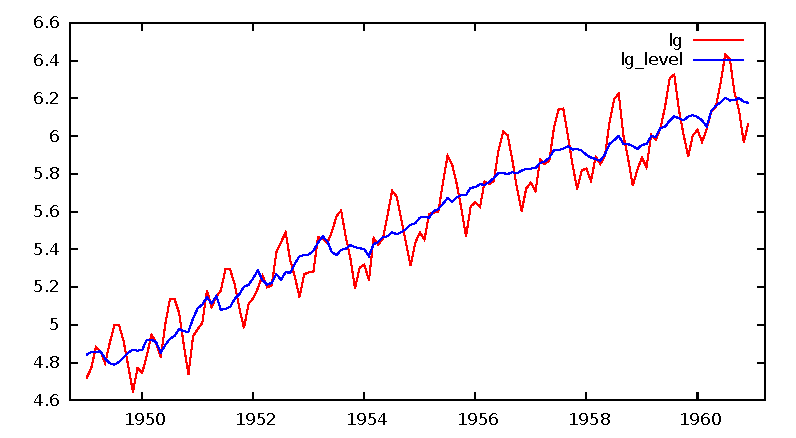
\includegraphics[scale=0.667]{ex1}
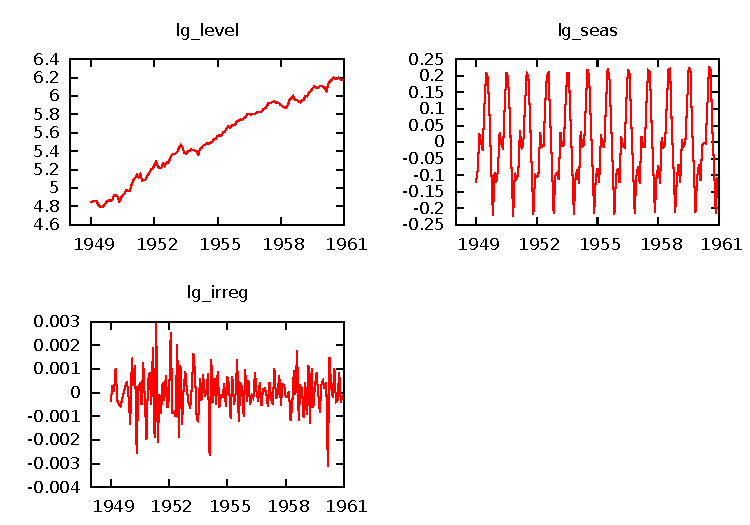
\includegraphics[scale=0.667]{ex2}
\end{figure}


Note that, differently from other programs, \app{StrucTiSM} reports
standard deviations rather than variances in the estimation
output.\footnote{It should also be noted that special care must be
  taken when reading the output, as the p-value reported cannot be
  interpreted as a proper test for zeroing the corresponding
  parameter. The reason is that a test for $\sigma = 0$ implies the
  evaluation of the log-likelihood and its derivatives at a point on
  the frontier of the parameter space, so usual asymptotics don't
  apply. See \cite{Pelagatti2015}, page 131.}

\begin{code}
Structural model for lg, 1949:01 - 1960:12 (T = 144)

                    coefficient   std. error     z     p-value 
  -------------------------------------------------------------
  Irregular         0.0113924     0.00567347   2.008   0.0446   **
  Trend             0.0264475     0.00359817   7.350   1.98e-13 ***
  Seasonal (dums)   0.00800572    0.00273532   2.927   0.0034   ***

Average log-likelihood = 1.27187

Specification:

Stochastic trend, no slope, dummy seasonals (stoch.),
irregular component  
\end{code}
and the plots are shown in figure \ref{fig:airline}.

The following example, instead, analyses the Nile data, the canonical
example employed in all the articles contained in the special issue of
the \emph{Journal of Statistical Software} devoted to state-space
modelling (see \cite{JSS2011}). It shows how to build a confidence
band around a smoothed state and draw it:

\begin{figure}[htb]
  \caption{LL model on the Nile data}
  \label{fig:Nile}
  \centering
  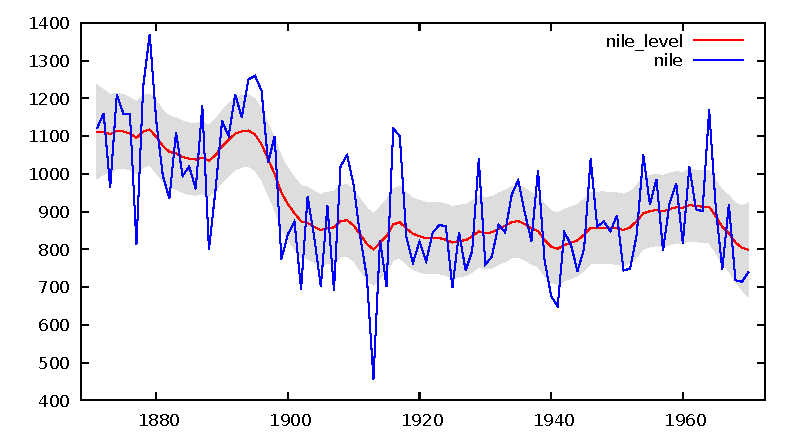
\includegraphics[scale=0.71]{nile_example}
\end{figure}

\begin{code}
include StrucTiSM.gfn 
open nile.gdt
LL = STSM_setup(nile,1,1,0,0)
STSM_estimate(&LL)
X = STSM_components(LL, 1)
list Plot = nile_level nile
plot Plot
    options time-series with-lines
    option band=nile_level,nile_level_se,1.96 
    option band-style=fill
end plot --output=display
\end{code}

\noindent
which produces what you see in figure \ref{fig:Nile}.

\subsection{Forecasting}
\label{sec:fcast}

For a thorough exposition of the approach we follow, the best
reference is probably section 4.11 in \cite{DK2012}. In brief,
forecasting on the basis of an already estimated model is performed
by running the Kalman filter on that model, in which a suitable number
of missing observaions are appended to the dependent variable.

The function that the package provides for this purpose is called
\cmd{STSM\_fcast} and it works by adding two new items to a model
bundle: both are vectors with $h$ elements, where $h$ is the desired
forecast horizon. They are contained under the names \texttt{fcast}
and \texttt{fcastvar}, and contain the point forecasts and their
variances, respectively. (Forecast variances do not take into 
account parameter uncertainty.)

By default, the function prints out the point forecasts and the
corresponding standard errors; this behaviour can be turned off by
providing 0 as the third parameter to the function (see section
\ref{sec:funcdoc}).

For example, the following script
\begin{code}
set verbose off
include StrucTiSM.gfn
open nile.gdt --quiet 

# estimate a local level model on the Nile data
model = STSM_setup(nile, 1, 1, 0, 0) 
# estimate silently
scalar err = STSM_estimate(&model, 0)

# forecast
STSM_fcast(&model, 4)
\end{code}

should produce this output
\begin{code}
Out of sample forecast for nile

   horizon    forecast    std.err.

         1     798.368     143.527
         2     798.368     148.557
         3     798.368     153.422
         4     798.368     158.138
\end{code}

Slightly more elaborate examples are provided in the
\texttt{forecasting.inp} script, in the examples directory. If
necessary, you can also obtain forecasts for the latent states, by
passing a fourth Boolean parameter. Again, see section \ref{sec:funcdoc} for
more details.

\subsection{Interpolation of missing values}
\label{sec:gapfill}

One thing state-space models are quite good at is interpolating
missing values (provided, of course, that the statistical model fits
the data reasonably well). As a consequence, it is easy to use a
structural model as a fancier alternative to crude interpolation
methods like the ones provided in the \verb|gap_filler| function, that
is contained in the \texttt{extra} addon to gretl.

The script below provides an example with Box and Jenkins' ``airline''
series, in which we artificially create a few gaps first and then fit
a Basic Structural Model to recover the missing entries.

\begin{code}
set verbose off
include StrucTiSM.gfn

# use Box and Jenkins' airline series
open bjg.gdt --quiet

# create a few artificial gaps
gappy = lg
smpl 1954:3 1955:6
gappy = NA
smpl full

# fit a Basic Structural model to the gappy series
m = BSM(gappy)

# fill in the gaps
gappy_filled = ok(gappy) ? gappy : gappy_level + gappy_seas

# compare original and reconstructed series
gnuplot gappy_filled lg --with-lines --time-series --output=display  
\end{code}

Running the above script above should produce the following output and
the plot depicted in figure \ref{fig:gappy}.

\pagebreak[4]

\begin{figure}[htbp]
  \centering
  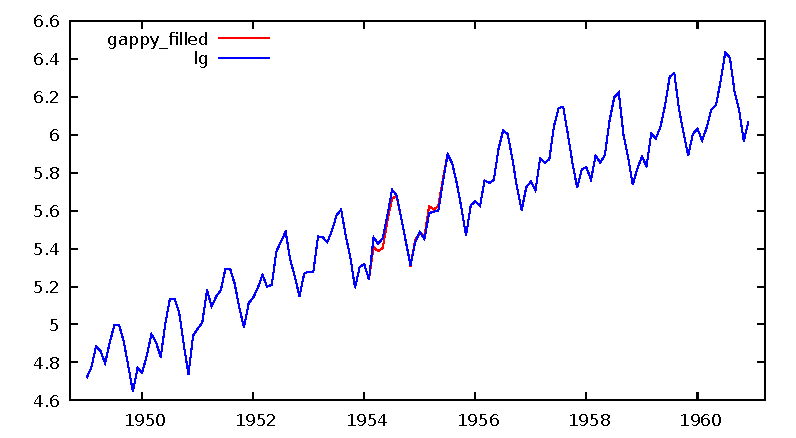
\includegraphics[scale=0.8]{gappy}
  \caption{Original and reconstructed airline data}
  \label{fig:gappy}
\end{figure}

\begin{code}
Structural model for gappy, 1949:01 - 1960:12 (T = 128)

                   coefficient  std. error       z      p-value 
  --------------------------------------------------------------
  Irregular        0.0110440    0.00656742   1.682      0.0926   *
  Trend            0.0293437    0.00415215   7.067      1.58e-12 ***
  Slope            4.17805e-08  0.000568305  7.352e-05  0.9999  
  Seasonal (dums)  0.00718025   0.00271764   2.642      0.0082   ***

Average log-likelihood = 1.60974


Specification:

Stochastic trend, stochastic slope, dummy seasonals (stoch.),
irregular component
\end{code}

\subsection{Exogenous variables}
\label{sec:exovar}

You may include exogenous regressors in your model. In this case
equation (\ref{eq:measuremment}) becomes
\begin{equation}
  \label{eq:exovar}
  y_t = x_t ' \beta + \mu_t + s_t + \varepsilon_t
\end{equation}
An example is given in the dedicated directory, where we use the
dataset made popular by \cite{Harvey1986} on the effects of seat belt
legislation in UK road fatalities. The file's name is
\verb|roadacc.inp|, and it contains a specification akin to the one
presented in \cite{CK2007}, section 7.2.

Please note that, as yet, models without stochastic components cannot
include exogenous variables. Use OLS for that.

\paragraph{Forecasting with exogenous variables}
When the model includes exogenous variables, forecasting is somewhat 
complicated by the requirement of having valid observations for those
non-modelled varaibles in the range of the forecasting horizon. How
this data handling is performed depends on whether the GUI or the 
scripting interface is used.

As explained in the forecasting section \ref{sec:fcast}, when using the 
GUI, the initially active sample must contain the forecast range. The 
StrucTiSM package then shortens the sample for estimation automatically, 
and this approach also covers the inclusion of exogenous variables by 
taking their forecast range values from the initial full sample. 
Obviously, those values have to exist to make forecasting with such a 
model possible.

The situation is a little bit different for the scripting interface. Here
estimation is always carried out for the currently active sample range,
because there is no way for the estimation function \texttt{STSM\_estimate()}
to know that a forecast is wanted later on. When calling the 
\texttt{STSM\_forecast()} function afterwards, the user must make sure that
the active sample at that point also covers the desired forecast range 
as indicated by the horizon argument. This is different from the situation
without exogenous variables, the reason being that the needed exogenous values
for the forecast range would not be available for the function otherwise.
Hence, the shortening of the active sample for estimation and the subsequent 
re-expansion for forecasting is the responsibility of the scripting user 
in this case. (The forecasting horizon can of course be shorter than the 
available post-estimation sample range, so that argument must still be 
specified.)

% Perhaps add a hint or a link to a new example file "forecasting_exo.inp"
% or something.    

\subsection{The GUI}
\begin{center}
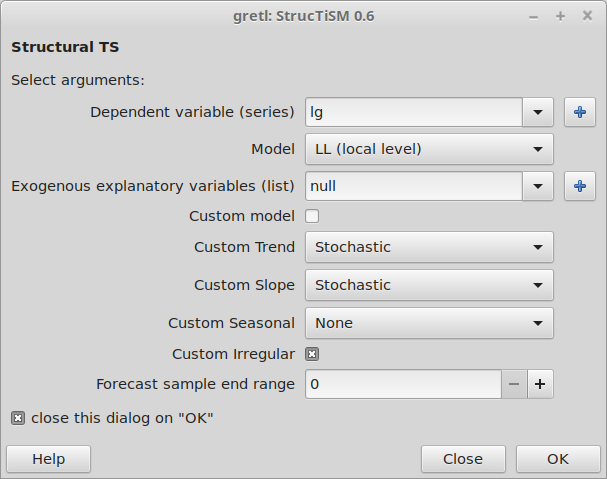
\includegraphics[width=0.66\textwidth]{GUI.png}
\end{center}

You access this window via the \emph{Model $>$ Time Series  $>$
  Structural TS} menu.

Things to note:
\begin{itemize}
\item You can select one of the three stock models from the drop-down
  menu, or put together your own combination, by ticking the ``custom
  model'' tick box. You may add exogenous variables via the
  appropriate box, either for stock models or custom ones.
\item After pressing ``OK'', estimation will be performed and the
  results displayed. If you click on the Graph button, a summary graph
  of the states will be produced.
\item The ``Save bundle content'' icon gives you access to the
  individual bundle elements, which include the smoothed states, the
  system matrices, and more.
\item You can save the model bundle by clicking the Save button in the
  output window. After that, you can extract the components by
  applying the \cmd{STSM\_components} function to the bundle you just
  saved.
\item Since v0.6 there is an additional integer argument specifying
  the forecast horizon. If you set that to a positive value, the
  estimation sample will be shortened by that amount, and forecasts
  will be produced for the trailing observations. Thus, if you want to
  calculate truly out-of-sample forecasts via the GUI, you would need 
  to add extra (empty) observations to your dataset (menu Data/Add 
  observations; or through the scripting command \cmd{dataset addobs})
  before calling the StrucTiSM package.
\end{itemize}

%\clearpage

\section{Function list (in alphabetical order)}
\label{sec:funcdoc}

\begin{funcdoc}{BSM(series y, bool se, model *mod)}
  Estimates a Basic Structural Model of $y_t$ and returns a list
  holding the components.
  \begin{itemize}
  \item \texttt{y}, the dependent variable
  \item \texttt{se}, include in the list also the estimated standard
    errors for the smoothed states (optional, default=no)
  \item \texttt{mod}, if not null, contains the estimated model upon
    successful completion
  \end{itemize}
\end{funcdoc}

\begin{funcdoc}{LLT(series y, bool se, model *mod)}
  Estimates a Local Linear Trend model of $y_t$ and returns a list
  holding the components.
  \begin{itemize}
  \item \texttt{y}, the dependent variable
  \item \texttt{se}, include in the list also the estimated standard
    errors for the smoothed states (optional, default=no)
  \item \texttt{mod}, if not null, contains the estimated model upon
    successful completion
  \end{itemize}
\end{funcdoc}

\begin{funcdoc}{STSM\_components(bundle mod, bool se)}
  Extracts the states to a list of series.
  \begin{itemize}
  \item \texttt{mod}, the estimated model
  \item \texttt{se}, include in the list also the estimated standard
    errors for the smoothed states (optional, default=no)
  \end{itemize}
\end{funcdoc}

\begin{funcdoc}{STSM\_estimate(bundle *mod, int verbose, int mapping,
    int vcvmethod)}
  Estimates the variances of the model and performs the state
  smoothing. The arguments are:
  \begin{itemize}
  \item \texttt{mod}, pointer to a bundle created via \cmd{STSM\_setup}
  \item \texttt{verbose}, verbosity (optional, default=1),
  \item \texttt{mapping} type of reparametrisation: 0 = Variances, 1 =
    Std. Dev (default), 2 = logarithm
  \item \texttt{vcvmethod} 0 = OPG, 1 = Hessian (default), 2 = QML
  \end{itemize}

  Returns an error code.
\end{funcdoc}

\begin{funcdoc}{STSM\_fcast(bundle *mod, int horizon, bool verbose,
    bool do\_states)}
  Forecasts the dependent variable and stores results into the bundle
  as \texttt{fcast} and \texttt{fcastvar}. The arguments are:
  \begin{itemize}
  \item \texttt{mod}, pointer to a bundle created via
    \cmd{STSM\_setup}; it must contain estimation results.
  \item \texttt{horizon}, an integer with the forecasting horizon. If
    0 or omitted, a ``sensible'' default based on current periodicity
    is used. 
  \item \texttt{verbose} Boolean. If non-zero, a printout is given
    with point forecasts and associated standard errors (default = yes).
  \item \texttt{do\_states} Boolean. If non-zero, the predicted values
    for the unobservable components are also stored into the bundle
    \texttt{mod} under the names \texttt{sfcast} and
    \texttt{sfcastvar}.
  \end{itemize}
  
  Returns an error code.

  \textbf{NOTE:} Models with exogenous variables are supported since version
    0.65, under the 
    obvious condition that those variables must have known values over the 
    forecasting horizon.
  
\end{funcdoc}

\begin{funcdoc}{STSM\_printout(bundle *mod)}
  Prints out the estimates.
\end{funcdoc}

\begin{funcdoc}{STSM\_setup(series y, bool epsilon, int trend, 
      int slope, int seasonal, list X)}
  Returns an initialised bundle. The arguments are:
  \begin{itemize}
  \item \texttt{y}, the dependent variable
  \item \texttt{epsilon}, Boolean, presence of $\varepsilon_t$ in
    eq. (\ref{eq:measuremment}) (optional, default=yes),
  \item \texttt{trend} type of trend: 1 = stochastic, 2 =
    deterministic (optional, default=1),
  \item \texttt{slope}  0 = none, 1 = stochastic, 2 =
    deterministic (optional, default=1),
  \item \texttt{seasonal} Seasonal, 0 = none, 1 = stochastic with
    trigonometric terms, 2 = stochastic with dummies, 3 =
    deterministic dummies (optional, default = 2)
  \item \texttt{X} list, exogenous variables in the measurement
    equation (optional, default = null)
  \end{itemize}
\end{funcdoc}

\bibliography{ref}

\section*{Changelog}
\begin{center}
\begin{tabular}{rp{0.7\textwidth}}
  \hline
  \textbf{Version} & \textbf{Changes}\\
  \hline
  0.1 & Initial release \\
  0.2 & Several bug fixes (thanks to Silvia Rodriguez
        for her bug report); exogenous variables in the measurement equation; optional
        export of the variance series for the smoothed states;
        switch to LBFGS for optimisation.\\
  0.3 & Handling models with no stochastic latent states via OLS as
        ``special cases''.\\
  0.4 & Bump version requirement to avoid windows bug; changed plot
        titles in GUI; added some error checking.\\
  0.5 & Add \cmd{STSM\_fcast} and make it possible to retrieve the
        model bundle from shortcut functions.\\
  0.51 & Fix bug with forecasting with models with no irregular component.\\
  0.52 & Add subsection \ref{sec:gapfill}.\\
  0.53 & Fix bug with forecasting when horizon = 1. \\
  0.6  & Attempt forecasting support in the GUI. \\
  0.7 & (Nov 2021) Extend forecasting support to models with exogenous variables;
      require gretl 2020c for internal reasons. \\
  \hline
\end{tabular}
  
\end{center}
\end{document}

%%% Local Variables: 
%%% mode: latex
%%% TeX-master: t
%%% End: 
